\documentclass{article}

\usepackage{amsfonts}
\usepackage{graphicx}

\setlength\parindent{18pt}

\begin{document}


Textbook Section 1.1:

8) \[y'' + y = 3cos2x, y_1 = cos(x) - cos2x, y_2 = sin(x) - cos2x\]

% TODO: Find out if there is a better way of doing identation of a line
\indent \indent a)

\[\frac{dy_1}{dx} = -sin(x) + 2sin(2x)\]
\[\frac{d^2y_1}{dx^2} = -cos(x) + 4cos2x\]

\[y_1'' + y_1 = (-cos(x) + 4cos2x) + (cos(x) - cos2x) = 3cos2x.\]


\indent \indent b)

\[\frac{dy_2}{dx} = cos(x) + 2sin(2x)\]
\[\frac{d^2y_2}{dx^2} = -sin(x) + 4cos2x\]

\[y_2'' + y_2 = (-sin(x) + 4cos2x) + (sin(x) - cos2x) = 3cos2x.\]



15) \[y'' + y' - 2y = 0\]

\[Let \; y = e^{rx}\]
\[ where \; r \in \mathbb{R} \; is \; a \; constant.\]
\[y' = re^{rx}\]
\[y'' = r^2e^{rx}\]

\[r^2e^{rx} + re^{rx} - 2re^{rx} = 0\]
\[(r^2 + r - 2)e^{rx} = 0\]
\[r^2 + r - 2 = 0\]
\[(r-1)*(r+2) = 0\]
\[r = 1 \; or \; r = -2.\]



34) The accleration $\frac{dv}{dt}$ of a Lamborghini is proportional to the
  difference between 250 km/h and the velocity of the car.


\[\frac{dv}{dt} = \frac{250 - v}{t}\]
\[\frac{dv}{250-v} = \frac{dt}{t}\]
\[-ln(250-v) = ln(t) + C\]
We discard the absolute value sign on $ln$ since we only care about
non-negative time and non-negative velocity.
\[\frac{1}{250-v} = t + C\]
\[250-v = \frac{1}{t + C}\]
\[v = 250 - \frac{1}{t + C}\]
Assuming t is non-negative and v is non-negative, then C would have to be $\geq$ $\frac{1}{250}$.


\hspace{1cm}

Textbook Section 1.2:

6) \[\frac{dy}{dx} = x - y + 1\]


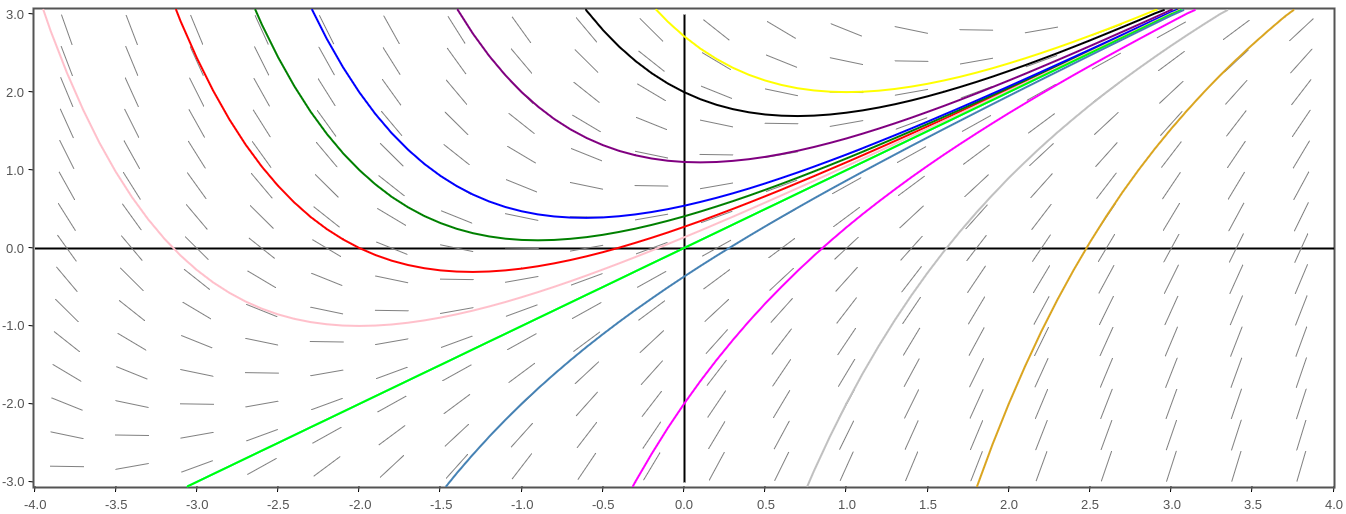
\includegraphics[width=\linewidth]{x_minus_y_plus_1}


7) \[\frac{dy}{dx} = sin(x) + sin(y)\]


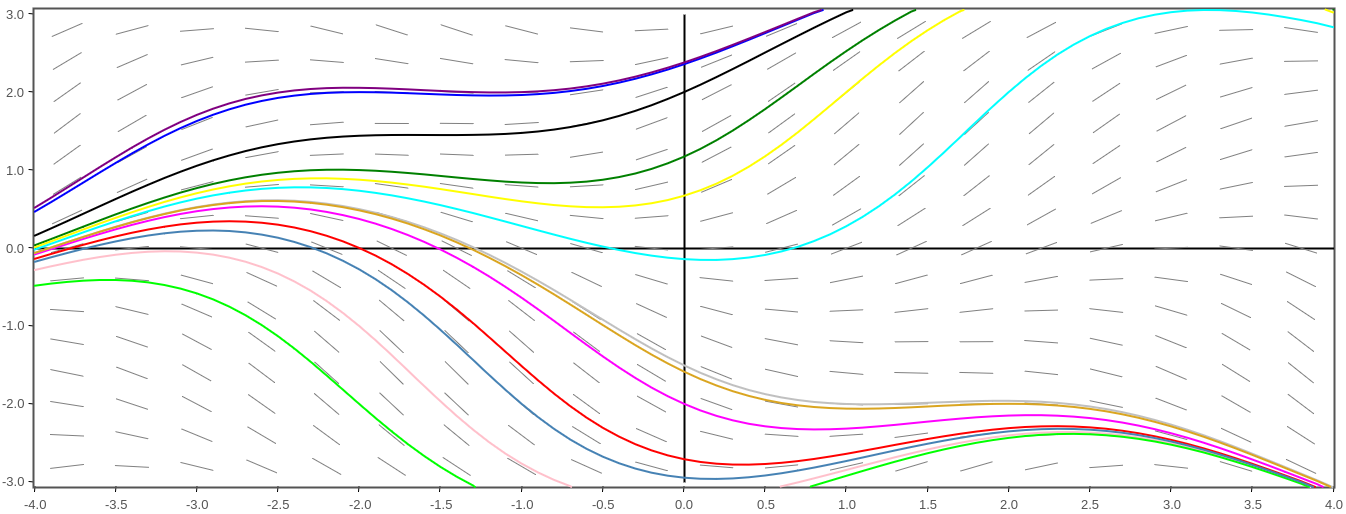
\includegraphics[width=\linewidth]{sinx_plus_siny}


9) \[\frac{dy}{dx} = x^2 - y - 2\]

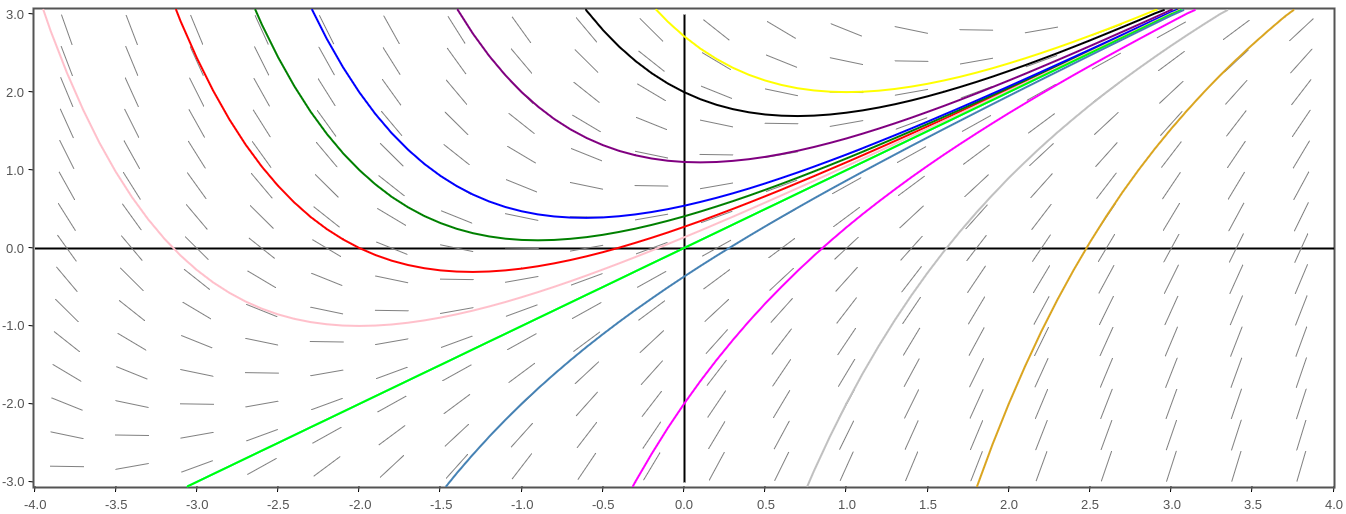
\includegraphics[width=\linewidth]{x_minus_y_plus_1}


24) \[y' = x + \frac{1}{2}y^2, y(-2) = 0, y(2) = ?\]

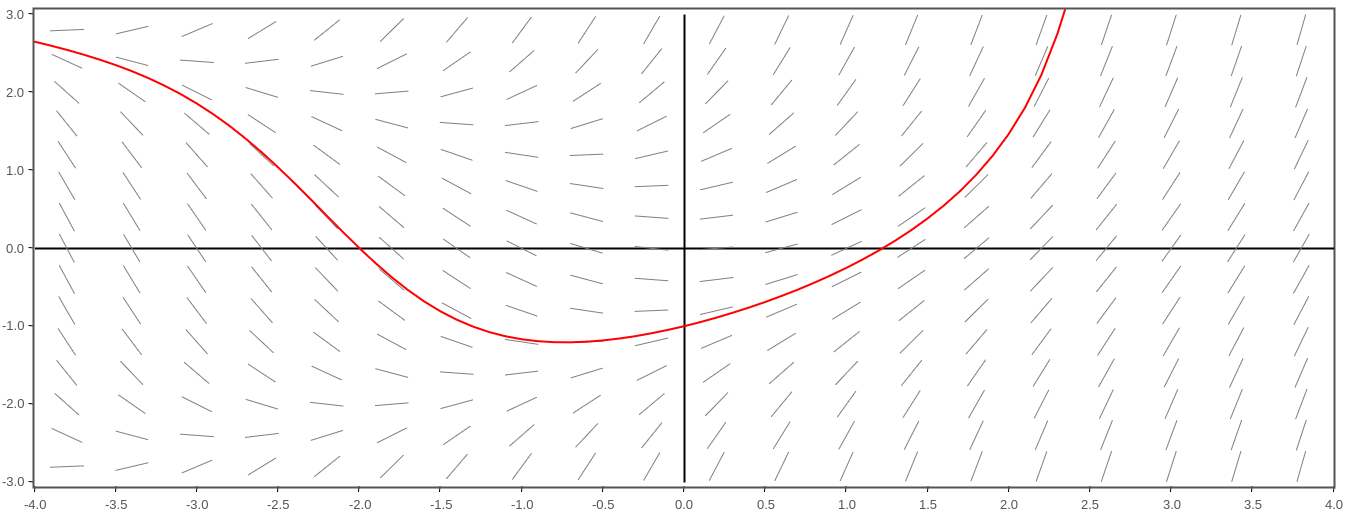
\includegraphics[width=\linewidth]{x_plus_one_half_y_squared}

\[y(2) \simeq 1.5\]


\hspace{1cm}

Textbook Section 1.4:

9) \[(1-x^2)\frac{dy}{dx} = 2y\]

\[(1-x^2)\frac{dy}{dx} = 2y \iff
\frac{dy}{2y} = \frac{dx}{1-x^2}\]

\[\int \frac{1}{2y}dy = \int \frac{1}{1-x^2}dx\]

\[\int \frac{1}{1-x^2}dx\]

\[1 - x^2 = (1-x)*(1+x)\]
\[\frac{1}{1-x^2} = \frac{A}{1-x} + \frac{B}{1+x}
= \frac{A*(1+x)}{(1-x)*(1+x)} + \frac{B*(1-x)}{(1-x)*(1+x)}\]
\[= \frac{A+Ax + B-Bx}{1-x^2}
= \frac{(A-B)x + (A+B)}{1-x^2}
= \frac{0*x + 1}{1-x^2}
\]
\[
\iff (A-B)x + (A+B) = 0*x + 1
\iff A-B = 0, A+B = 1
\]
\[A = B, 2A = 1 \iff A = 1/2\]

\[\int \frac{1}{1-x^2}dx
= \int \frac{1/2}{1-x}dx + \int \frac{1/2}{1+x}
\]
\[
= -\frac{1}{2}\int \frac{-1}{1-x} + \frac{1}{2}\int \frac{1}{1+x}
\]

\[
= -\frac{1}{2}ln|1-x| + \frac{1}{2}ln|1+x|
\]

\[\int \frac{1}{2y}dy = \int \frac{1}{1-x^2}dx\]
\[D = 2C\]
\[A = e^D\]
\[\iff \frac{1}{2}ln|y| = -\frac{1}{2}ln|1-x| + \frac{1}{2}ln|1+x| + C\]
\[\iff ln|y| = -ln|1-x| + ln|1+x| + D\]
\[\iff |y| = e^{ln(\frac{1}{|1-x|}) + ln|1+x| + D}\]
\[\iff |y| = e^{ln(\frac{1}{|1-x|})} * e^{ln|1+x|} * e^D\]
\[\iff |y| = \frac{1}{|1-x|} * |1+x| * e^D\]
\[\iff |y| = A\frac{|1+x|}{|1-x|}\]
\[\iff y = \pm A\frac{|1+x|}{|1-x|}\]

Now if we plug in for positive x, we will get:
\[y = \pm A*\frac{1+x}{1-(-x)}
\iff y = \pm A*\frac{1+x}{1+x}
\iff y = \pm A * 1
\iff y = \pm A\]

And for negative x, we will get:
\[y = \pm A*\frac{1+(-x)}{1-x}
\iff y = \pm A*\frac{1-x}{1-x}
\iff y = \pm A*1
\iff y = \pm A\]

So,
\[y = \pm A\]

Which works out if you plug it into the original ODE that we were given 
(note that D = 2C, which is why the constant of 2 appears on the rhs).


13) \[y^3 \frac{dy}{dx} = (y^4 + 1)cos(x)\]

\[y^3 \frac{dy}{dx} = (y^4 + 1)cos(x)\]
\[\iff \frac{y^3}{y^4+1}dy = cos(x) dx\]
\[\iff \int \frac{y^3}{y^4+1}dy = \int cos(x) dx\]
\[\iff \frac{1}{4}\int \frac{4y^3}{y^4+1}dy = \int cos(x) dx\]
\[\iff \frac{1}{4}ln|y^4 + 1| = sin(x) + C\]

Notice that $y^4 + 1$ is always positive,
so we can replace $|y^4 + 1|$ with $(y^4 + 1)$.

\[D = 4C\]
\[A = e^D\]

\[\frac{1}{4}ln(y^4 + 1) = sin(x) + C\]
\[\iff ln(y^4 + 1) = 4sin(x) + D\]
\[\iff y^4 + 1 = e^{4sin(x) + D}\]
\[\iff y^4 + 1 = A*e^{4sin(x)}\]
\[\iff y^4 = A*e^{4sin(x)} -  1\]
\[\iff y = \sqrt[4]{A*e^{4sin(x)} -  1}\]


22) \[\frac{dy}{dx} = 4x^3y - y, y(1) = -3\]

\[A = e^C\]

\[\frac{dy}{dx} = 4x^3y - y, y(1) = -3\]
\[\iff \frac{dy}{dx} = (4x^3 - 1)*y\]
\[\iff \frac{1}{y}dy = (4x^3 - 1)dx\]
\[\iff \int \frac{1}{y}dy = \int (4x^3 - 1)dx\]
\[\iff ln|y| = x^4 - x + C\]
\[\iff |y| = e^{x^4 - x + C}\]
\[\iff |y| = A*\frac{e^{x^4}}{e^x}\]
\[\iff y = \pm A*\frac{e^{x^4}}{e^x}\]

Notice that $\frac{e^{x^4}}{e^x}$ is always positive, so we can can rewrite this as:
\[y = A*\frac{e^{x^4}}{e^x}\]

Now, we have to find A.

\[y(1) = A*\frac{e^{1^4}}{e^1} = -3\]
\[A*\frac{e^{1^4}}{e^1} = A*\frac{e^1}{e^1} = A\]
\[\iff y(1) = A = -3\]

So,
\[A = -3\]
and
\[y = -3*\frac{e^{x^4}}{e^x}\]


54) A tank is shaped like a vertical cyclinder;
it initially contains water to a depth of 9ft,
and a bottom plug is removed at time t = 0 (hours).
After 1hr, the depth of the water has dropped to 4ft.
How long does it take for all the water to drain from the tank?

\[y(0) = 9\]
\[y(1) = 4\]
\[D = \frac{C}{2}\]

\[A = \pi r_1^2\]
\[g = 32\frac{ft}{s^2}\]
\[a = \pi r_2^2\]
\[k = a\sqrt[2]{2g}\]
\[A*\frac{dy}{dt} = -k\sqrt[2]{y}\]
\[\iff \frac{1}{\sqrt[2]{y}}dy = -kAdt\]
\[\iff \int y^{-\frac{1}{2}}dy = \int -kAdt\]
\[\iff 2y^{1/2} = -kAt + C\]
\[\iff \sqrt[2]{y} = \frac{-kA}{2}t + D\]
\[\iff y = (\frac{-kA}{2}t + D)^2\]
\[\iff y = \frac{k^2A^2}{4}*t^2 - kAD*t + D^2\]

\[y(0) = D^2 = 9\]
\[\iff D = 3\]

\[y = \frac{k^2A^2}{4}*t^2 - kAD*t + D^2\]
\[\iff y = \frac{k^2A^2}{4}*t^2 - kA*3*t + 9\]


\[y(1) = \frac{k^2A^2}{4} - kA*3 + 9 = 4\]
\[\iff k^2A^2 - kA*12 + 20 = 0\]

\[M = kA\]

\[k^2A^2 - kA*12 + 20 = 0\]
\[\iff M^2 - 12M + 20 = 0\]

\[\iff M = 10, M = 2
\iff M = 6 \pm 4\]

\[y = \frac{k^2A^2}{4}*t^2 - kA*3*t + 9\]
\[\iff y = \frac{(6 \pm 4)^2}{4}*t^2 - (6 \pm 4)*3*t + 9\]


Now that we have $y$, we need to find when the value of $t$ when $y = 0$.

\[y = \frac{(6 \pm 4)^2}{4}*t^2 - (6 \pm 4)*3*t + 9 = 0\]

Let's split this into two clauses ($M = 2$ and $M = 10$).

For $M = 10$:
\[y = \frac{(6 + 4)^2}{4}*t^2 - (6 + 4)*3*t + 9 = 0\]
\[\iff y = \frac{100}{4}*t^2 - 30*t + 9 = 0\]
\[\iff y = 100*t^2 - 120*t + 36 = 0\]
\[t = \frac{3}{5}\]

For $M = 2$:
\[y = \frac{(6 - 4)^2}{4}*t^2 - (6 - 4)*3*t + 9 = 0\]
\[\iff t^2 - 6*t + 9 = 0\]
\[t = 3\]

So, the tank will become empty at either $t = \frac{3}{5}$ or $t = 3$
as given by the equation $y = \frac{(6 \pm 4)^2}{4}*t^2 - (6 \pm 4)*3*t + 9$.




Custom Problems:

Problem 1.

\indent \indent a) Construct a slope field for $y' = y(1 - y)$
on the interval $-2 \leq x$, $y \leq 2$.

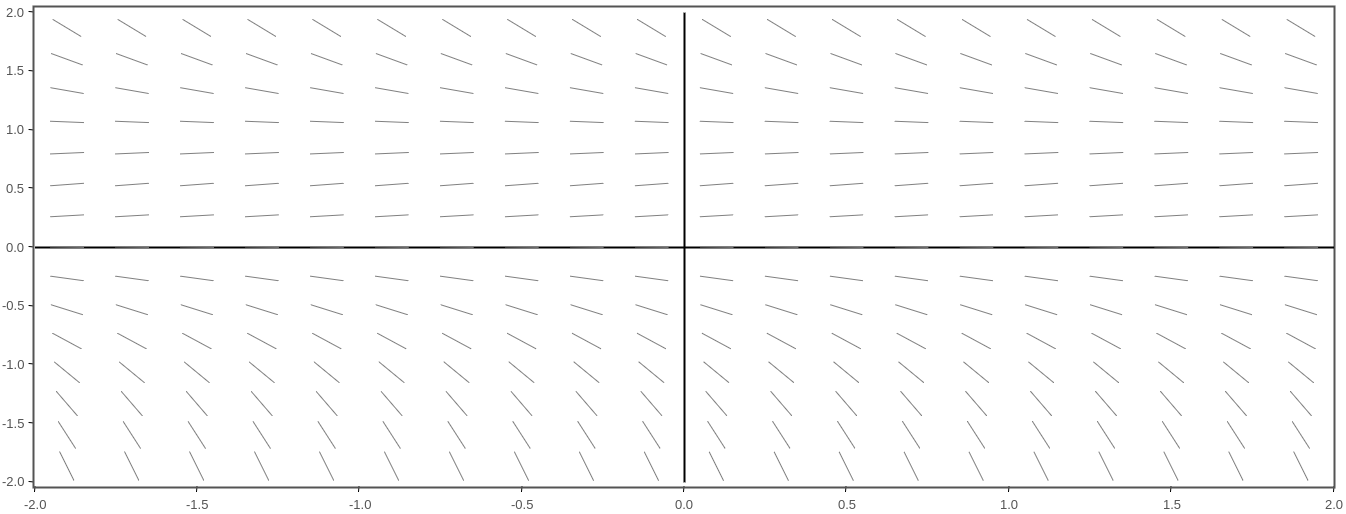
\includegraphics[width=\linewidth]{y_times_1_minus_y}


\indent \indent b)

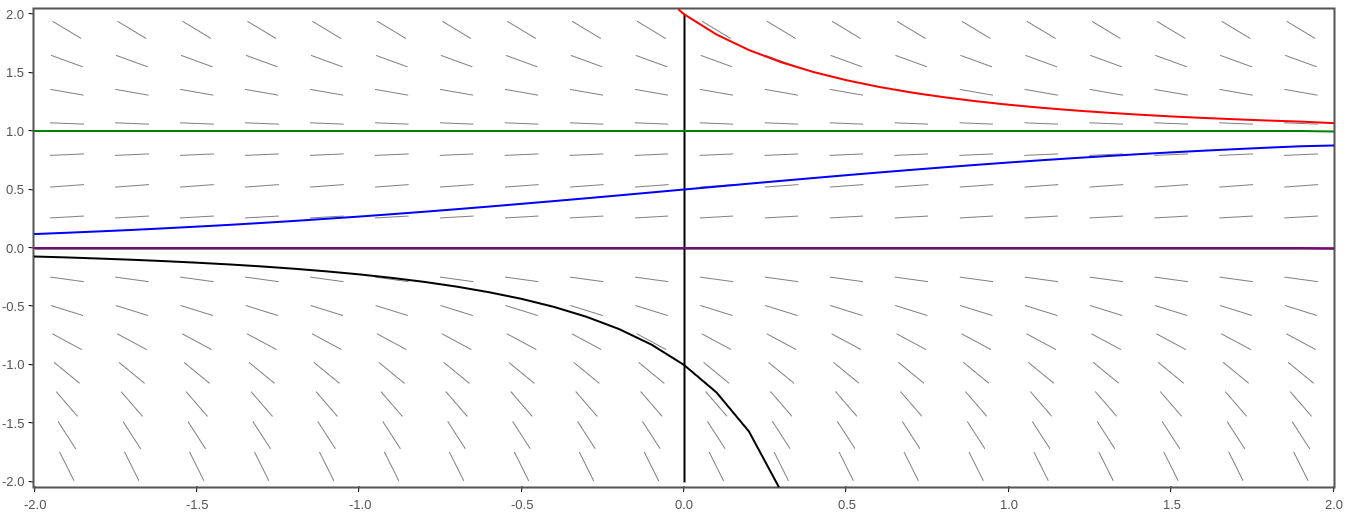
\includegraphics[width=\linewidth]{y_times_1_minus_y_with_points}


\end{document}
